\cotefile{157-5}
\scanpage{513}
\mspage{425}
% B01
4.15. \uline{Catégorie accessible sur une autre}.

% B02
\uline{Proposition} 4.15.1. Soit $f:E\unsure{\relbar|\longrightarrow} C$ un foncteur, avec $C$ \deleted{\unsure{essentiellement}} petite, \deleted{$E$ et $f$ \unsure{satisfaisant|satisfont} à la condition \unsure{la|H}.} On suppose de plus satisfaite la condition $H$ (p. 409), qu'on explicite \unsure{ici} sous la forme équivalente $H'$)

% B03
$H\unsure{'|^{*}}1)$ Pour tout $s\in\mathrm{Ob}\,C$, $E_s$ est accessible

% B04
$H'\deleted{\unsure{2}}3)$ Pour tt $\lambda\in\deleted{\unsure{\mathrm{Ob}}}\mathrm{Fl}\,C$, $\lambda:s\to t$, et pour tout $x_0\in\mathrm{Ob}\,E_s$, le foncteur
% B05
\[x_1\longrightarrow\mathrm{Hom}_{\lambda}(x_0,x_1):\quad E_t\unsure{\relbar|\longrightarrow}(\mathrm{Ens})\]
% B06
est accessible

% B07
\margin{\figure{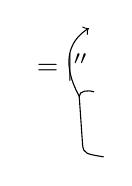
\begin{tikzpicture}[x=.27cm,y=.27cm]\node at (-.79,4.2) {$\unsure{=|''}$};\draw (1.15,0) .. controls (.35,.13) and (.2,.15) .. (.16,.55) -- (0,2.85) .. controls (0,3.12) and (.44,3.15) .. (.7,3.06);\draw[->] (0,2.85) .. controls (-1,4.7) and (-.25,5.6) .. (.45,6.05);\end{tikzpicture}}}

% B08
$H'\deleted{\unsure{3}}2)$ Pour tt $\lambda\in\mathrm{Fl}\,C$, $\lambda:s\to t$, existe un cardinal infini $\pi_\lambda$ tel que pour tt $x_1\in\mathrm{Ob}\,E_t$, le foncteur
% B09
\[x_0\longmapsto\mathrm{Hom}_{\lambda}(x_0,x_1):\quad E_s\longrightarrow(\mathrm{Ens})^\circ\]
% B10
est $\pi_\lambda$-accessible\deleted{\unsure{s}} ($E_s$ satisfaisant de plus \unsure{:|à} $L_{\pi_\lambda}$).

% B11
Alors \deleted{$E$ est accessible, et $f$ accessible \unsure{(pour} \inserted{\deleted{\unsure{satisfait},}} \illegible{3} \unsure{hypothèses|hypothèse}), \unsure{de façon plus précise},} les foncteurs d'inclusion $i_s:E_s\longrightarrow E$ sont accessibles. De plus, si $C$ est ``sans projecteurs'' (i.e si tout endom. $p$ d'un \unsure{objet} $s$ de $C$, tel que $p^2=p$, est l'identité), alors $E$ est accessible, et $p:E\to C$ est accessible.

% B12
Cela résulte des résultats plus précis

% B13
\deleted{\uline{Corollaire} 4.15.2. \unsure{a)} Soit \inserted{$s\in\mathrm{Ob}\,C$ et} $\pi_0$ un cardinal \deleted{\unsure{majorant les} \illegible{2} $E_s$ tel que : $\pi_0$} \inserted{\unsure{$E$ et $f$ satisfont}} tel que \unsure{a)} $\pi_0$ majore les $\pi_\lambda$ intervenant dans $H'3)$, pour $\lambda:s\to t$ (\unsure{flèche} de source \unsure{s})}

% archive sheet number: 512
